\section{Generics e Collection}
I generics sono stati introdotti in Java 5 e sono simili ai template di classe e di funzione del C++. In Java si usa la terminalogia \textbf{classe generica} e \textbf{metodo generico}.
I generics consentono di scrivere codice meno verboso evitando pericolosi cast di tipi, e permettendo di creare algoritmi generici (ovvero basati sui generics).

La definizione utilizza un tipo parametrico T che deve essere specificato quando si vuole usare un’istanza di quel template di classe/
interfaccia, mentre per i metodi viene dedotto dal compilatore. Il tipo T non può essere un primitivo; vengono accettati solo tipi classe e interfaccia.
Per definire un generic si usano le parentesi angolari:
\begin{lstlisting}
public class Classe <T,Z> { }

public interface Interfaccia <T> { }
 
public <T> void f(T[] array ) { }
\end{lstlisting}
Un metodo statico di una classe generica che utilizza un tipo parametrico deve essere un metodo generico o si ha un errore di compilazione.
\begin{lstlisting}
public class Classe <T >{

	public static <T> void m(T[] arg ) { }
 }
\end{lstlisting}
Se un generic viene esteso o implementato, deve essere indicato il tipo esplicitamente nella segnatura.

\subsection{Classi generiche}

La classe \textit{ArrayList} della libreria, ad esempio, è generica, cioè è stata dichiarata usando un parametro di tipo \textit{T}.

\begin{figure}[H]
\centering
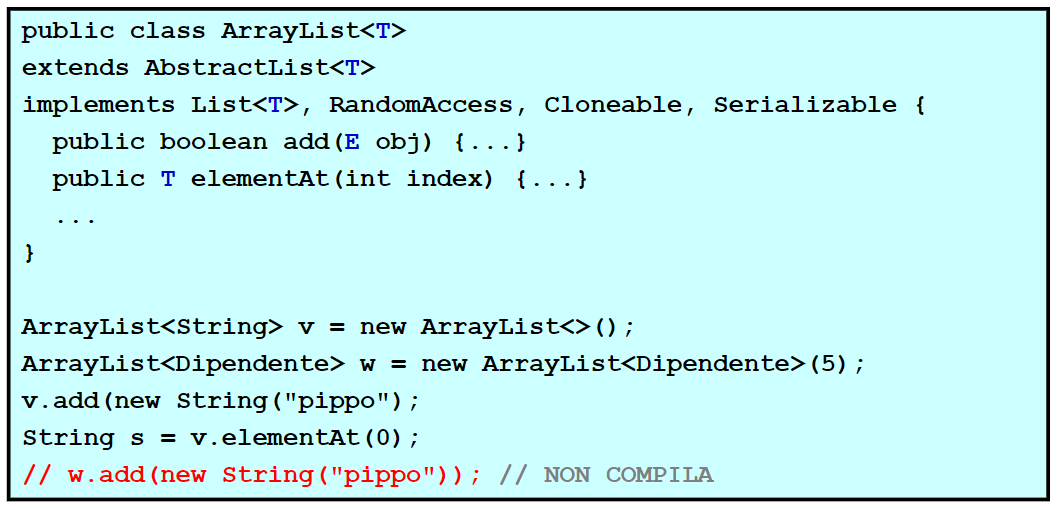
\includegraphics[scale=0.6]{images/classiGeneriche1}
\caption{Generics - ArrayList\label{fig:UC3}}
\end{figure}

Qui vediamo che la classe ArrayList è generica perché accetta un parametro chiamato \textbf{T} e questo verrà usato al suo interno per definire metodi e variabili. Come si può vedere, se T fosse stata di tipo String, allora ci sarebbe un \textit{tipaggio forte} e nessun altro tipo sarebbe stato accettato.
In pratica, una volta definito il tipo del parametro, bisognerà sempre tenere presente che verrà usato quel tipo. Se la classe sopra, cioè Dipendente, fosse stata una superclasse, non sarebbe stato comunque accettabile fornire una sua sottoclasse al metodo \textit{add()}. Non centra l’ereditarietà, bisogna che il tipo sia uguale.

I parametri di tipo di un generics possono essere istanziati a classi ed interfacce ma non a tipi primitivi.
Prima dei generics, la classe \textit{Vector} (thread-safe \textit{ArrayList}) sfruttava l'Object:

\begin{figure}[H]
\centering
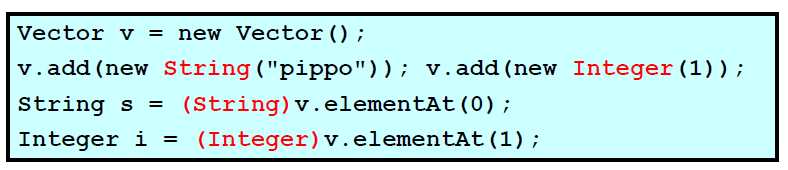
\includegraphics[scale=0.6]{images/classiGeneriche2}
\caption{Prima dei Generics - Vector\label{fig:UC3}}
\end{figure}
Posso inserire qualsiasi tipo di oggetto ma devo sapere cosa si va a pescare (cast specifico a run-time) per poter sfruttare l'oggetto. \textbf{{\color{error}Potenziale disastro a run-time!}}

Esempio di una semplice classe generica \textit{Coppia<T,S>}:
\begin{figure}[H]
\centering
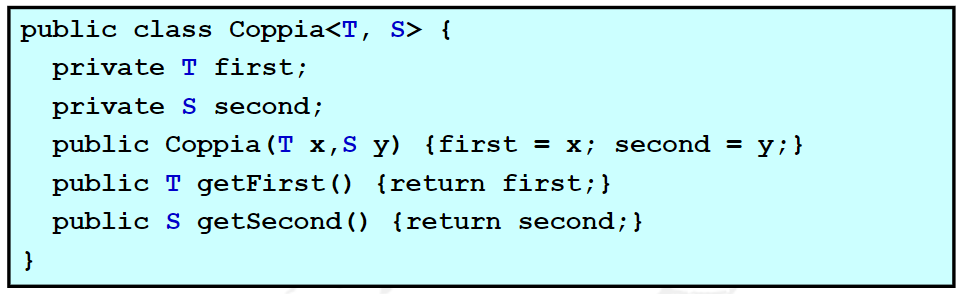
\includegraphics[scale=0.6]{images/classiGeneriche3}
\caption{Generics - classe generica\label{fig:UC3}}
\end{figure}

Ecco un esempio di classe con due parametri generici. Quando si istanzia il tipo, basta fornire i tipi al posto dei parametri e il compilatore dedurrà automaticamente i tipi da sostituire alle variabili. Quindi:

\begin{lstlisting}
var c = new Coppia<Integer, Double>(3, 7)();
\end{lstlisting}
Importante notare che i parametri generici possono essere istanziati a classi e interfacce ma {\color{error}NON} a tipi primitivi.Per questo motivo è stata usata la classe wrapper Integer al posto di un int nel costruttore. Grazie al boxing del tipo, è stato possibile passare un int all’Integer. Notare che questo codice non compila:
\subsection{Metodi generici}
Un metodo generico è un metodo che ha una o più variabili di tipo. Se non vi fosse la possibilità di scrivere il metodo in forma
generica, per adempiere allo stesso scopo si dovrebbe ricorrere al meccanismo dell’overloading dei metodi, che comporta la necessità di scrivere tanti metodi che eseguono lo stesso compito su tipi di dato differenti. 
Quando si invoca un metodo generico non si devono specificare i tipi effettivi da usare al posto dei parametri di tipo: si invoca semplicemente il metodo con i parametri appropriati e il compilatore dedurrà corrispondentemente i tipi da usare per i parametri. Bisogna usare metodi generici ogniqualvolta si può. Se è possibile, conviene utilizzare un metodo generico al posto dell'intera classe. Se un metodo è statico non avrà alcun accesso ai parametri generici della classe. Se serve che esso sia generico, serve dichiararlo esplicitamente usando un altro tipo.
\begin{lstlisting}
public class C<T>{
	public static void print(T[] a) {
	
	}
} 
//Non compila: Cannot make a static reference to non-static type T
\end{lstlisting}
\begin{lstlisting}
public class C<T>{
	public static <E>void print(E[] a) {
	...
	}
}//OK!
\end{lstlisting}
\subsubsection{Prima delle Generics}
Vediamo alcuni esempi di come venivano scritti le classi senza l'utilizzo delle generics:
Il primo esempio che vediamo è stato preso dal libro Java 8 Guida Completa di Pellegrino Principe
Questa è la versione senza Generics:

\begin{lstlisting}
package com.pellegrinoprincipe;
class PrintArray
{
	public PrintArray() {}
	public void printArray(Integer el[]) // stampa un array di interi
	{
		for (Integer i : el)
		System.out.print(i + " ");
	}
	public void printArray(Double el[]) // stampa un array di double
	{
		for (Double i : el)
		System.out.print(i + " ");
	}
	public void printArray(Character el[]) // stampa un array di caratteri
	{
		for (Character i : el)
		System.out.print(i + " ");
	}
}
public class PrintArrayClient
{
	public static void main(String[] args)
	{
		PrintArray pa = new PrintArray();
		Double d[] = { 11.1, 11.2 };
		Integer i[] = { 12, 13 };
		Character c[] = { 'a', 'b'};
		System.out.print("[ ");
		pa.printArray(d);
		pa.printArray(i);
		pa.printArray(c);
		System.out.print("]");
	}
}

//output : [ 11.1 11.2 12 13 a b ]
\end{lstlisting}
Il codice sopra crea una classe denominata PrintArray con tre metodi in overloading che permettono di stampare tutti gli elementi di un array di tipo differente.

 Nella classe PrintArrayClient si creano un oggetto di tipo PrintArray e tre riferimenti di oggetti array che contengono rispettivamente valori di tipo double, int e char. Nell'assegnamento dei valori agli array viene sfruttato \textit{autoboxing} e \textit{autounboxing} (vedi §4.1). 

L'output sarà sempre diverso, perchè a seconda del tipo di valore passato come argomento, il compilatore invocherà il corrispettivo metodo, grazie all'overloading. \newline

Vediamo adesso quanto semplice diventa il codice con l'utilizzo delle Generics:
\begin{lstlisting}
package com.pellegrinoprincipe;
class PrintArrayGeneric
{
	public PrintArrayGeneric() {}
	public <E> void printArray(E el[])
	{
		for (E i : el) // stampa in modo generico gli elementi 
		//dell'array di differente tipo
		System.out.print(i + " ");
	}
}

public class PrintArrayGenericClient
{
	public static void main(String[] args)
	{
		PrintArrayGeneric pag = new PrintArrayGeneric();
		Double d[] = { 11.1, 11.2 };
		Integer i[] = { 12, 13 };
		Character c[] = { 'a', 'b' };
		String s[] = { "sono", "una", "stringa" };
		System.out.print("[ ");
		pag.printArray(d);
		pag.printArray(i);
		pag.printArray(c);
		pag.<String>printArray(s); // sintassi alternativa di invocazione 
		//di un metodo generico
		System.out.print("]");
	}
}
//output: [ 11.1 11.2 12 13 a b sono una stringa ]
\end{lstlisting}
Come possiamo notare il codice si riduce drasticamente. Abbiamo infatti scritto un solo metodo, rispetto ai 3 del codice precedente.

\textbf{In dettaglio}:  il metodo printArray ha, nella sezione di dichiarazione dei parametri di tipo, il tipo \textbf{E}, che è utilizzato poi come tipo del parametro formale nella lista dei parametri del metodo (E el[]) e poi come tipo della variabile locale nel ciclo for (E i). Notiamo, inoltre, che nella classe PrintArrayGenericClient abbiamo aggiunto un array di oggetti String e l’abbiamo fatto stampare sempre dal metodo printArray. Quest’aggiunta, tuttavia, non ha invalidato la corretta compilazione del programma.
Infatti, poiché printArray è un metodo generico, non è stato necessario scrivere nella classe PrintArrayGeneric il corrispondente metodo in overloading che accettasse un argomento di tipo array di String (cosa che, invece, avremmo dovuto fare se il linguaggio non avesse supportato i generici).

Infine, è interessante evidenziare l’istruzione \textit{pag.<String>printArray(s)}, che mostra un modo alternativo per invocare un metodo generico che si concretizza nel passare il tipo effettivo tra le parentesi angolari < > prima del nome del metodo stesso. Tuttavia tale sintassi non è necessaria; infatti si può tranquillamente omettere di scrivere il tipo tra le parentesi angolari, poiché il compilatore è in grado di “capirlo” autonomamente analizzando il tipo passato come argomento, come mostrato per le altre invocazioni del metodo printArray (type inference).

\textbf{type inference} : è la capacità del compilatore di determinare automaticamente il tipo di argomento di un metodo generico. Il compilatore è in grado di inferire (dedurre) in autonomia il tipo di argomento quando il risultato di un'invocazione di metodo è passato come argomento a un altro metodo (\textit{inference in argument position} o \textit{inference in method context})

\subsection{Vincoli sui tipi delle variabili e Wildcards}
Spesso è necessario specificare quali tipi possano essere usati in una classe generica oppure in un metodo generico. Ad esempio, in un metodo generico \textit{T min(T[] a)} che trova il valore minimo presente in un array:


\begin{lstlisting}
public static <T> T min (T[] a) {
T x = a[0];
for(int i=1; i<a.lenght; ++i) 
	if(a[i] < x) 
		x=a[i];
		
	return x;
}
\end{lstlisting}
Il compilatore non può applicare l'operatore < perchè non sa nulla su T, sa solamente che è un tipo che verrà istanziato. Non può sapere l’effetto dell’operatore sul tipo T perché non può sapere cosa diventerà T (Integer, Double, una classe, un’interfaccia...). Per risolvere il problema si può fare così:

\begin{lstlisting}
public static <T extends Comparable<T>> E min (E[] a){
	E x = a[0];
	for(int i = 1; i<a.length; ++i)
		if(a[i].compareTo(x) < 0)
			x=a[i];
	return x;
}
\end{lstlisting}


